\section{Generate report}
\label{group____generate__report}\index{Generate report@{Generate report}}
Generate a report to show the states of OCG modules.  




Collaboration diagram for Generate report:\nopagebreak
\begin{figure}[H]
\begin{center}
\leavevmode
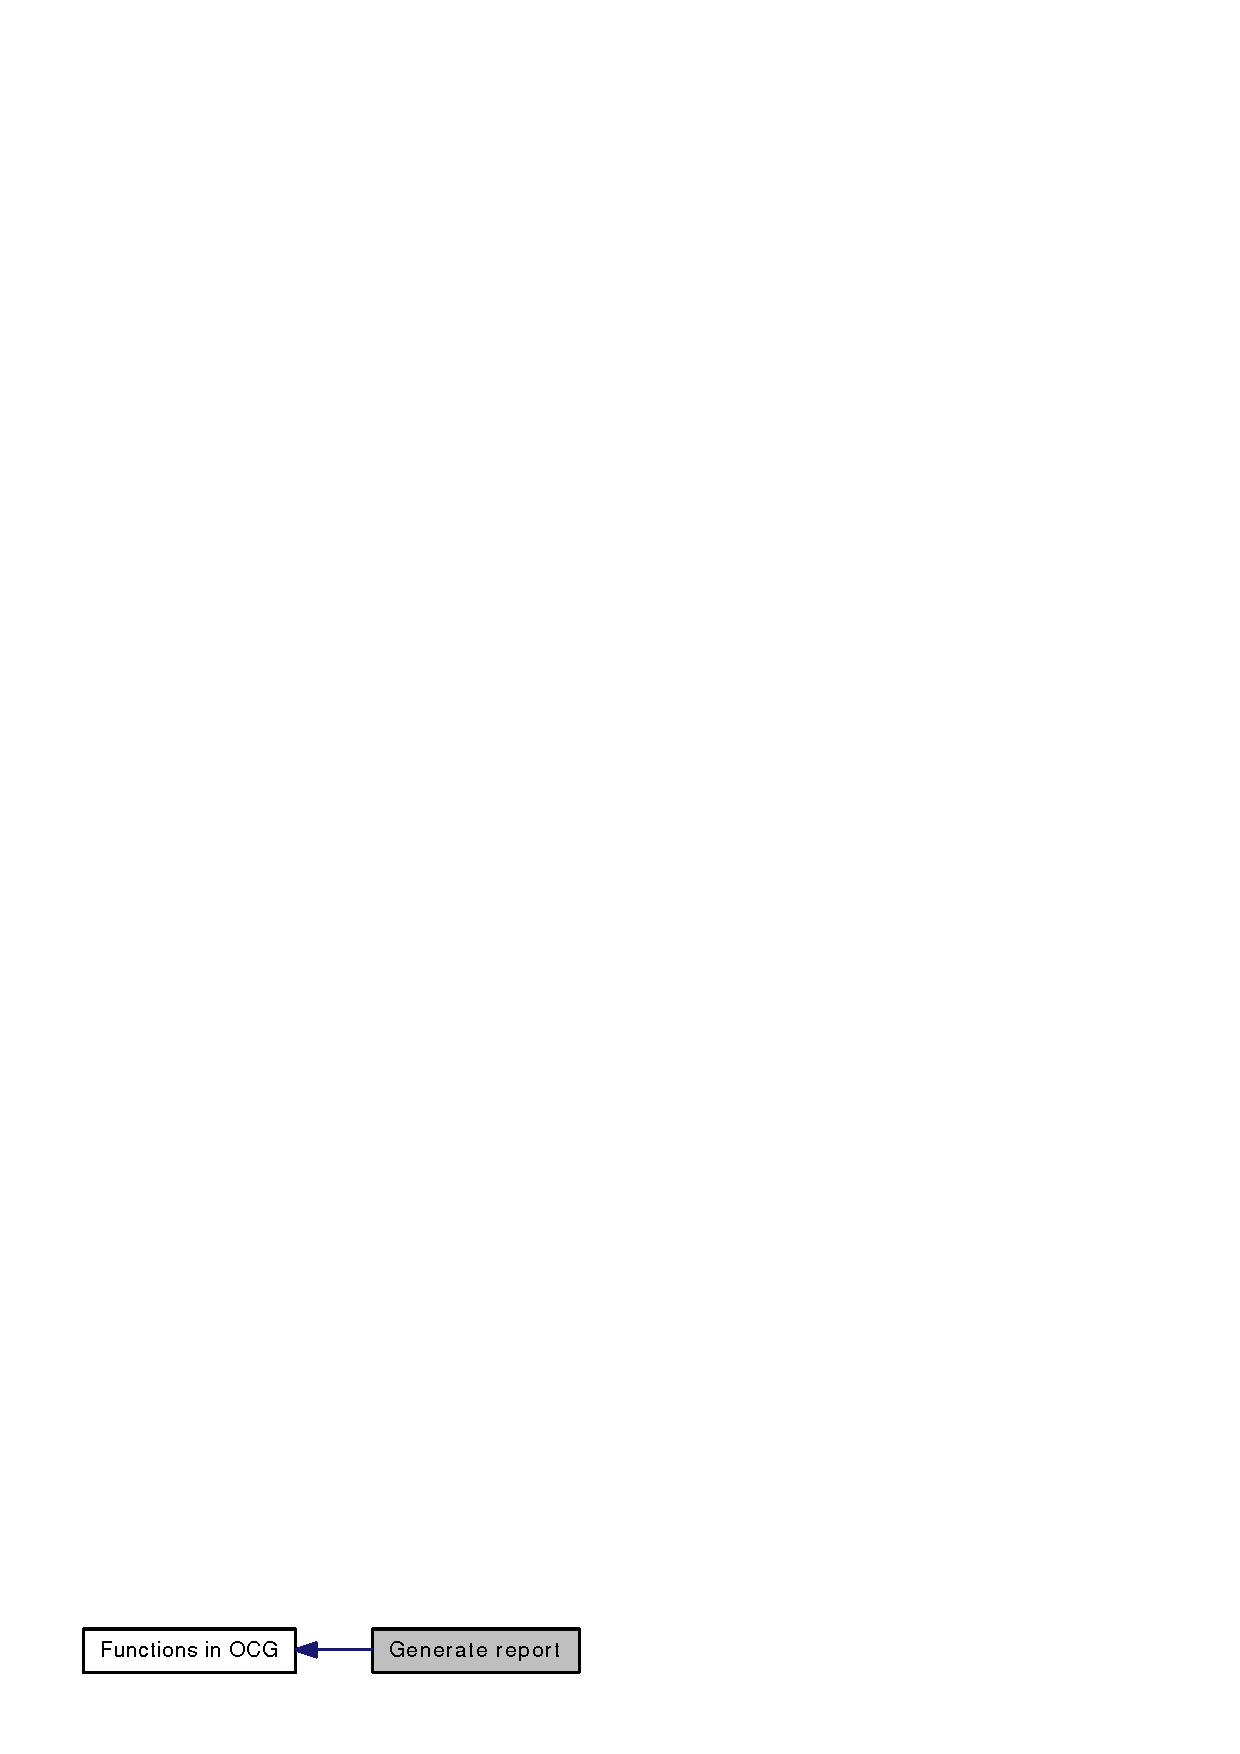
\includegraphics[width=141pt]{group____generate__report}
\end{center}
\end{figure}
\subsection*{Functions}
\begin{CompactItemize}
\item 
int {\bf generate\_\-report} (char dst\_\-dir[DIR\_\-LENGTH\_\-MAX], char filename[FILENAME\_\-LENGTH\_\-MAX])
\end{CompactItemize}


\subsection{Detailed Description}
Generate a report to show the states of OCG modules. 

\subsection{Function Documentation}
\index{\_\-generate\_\-report@{\_\-generate\_\-report}!generate\_\-report@{generate\_\-report}}
\index{generate\_\-report@{generate\_\-report}!_generate_report@{\_\-generate\_\-report}}
\subsubsection[{generate\_\-report}]{\setlength{\rightskip}{0pt plus 5cm}int generate\_\-report (char {\em dst\_\-dir}[DIR\_\-LENGTH\_\-MAX], \/  char {\em filename}[FILENAME\_\-LENGTH\_\-MAX])}\label{group____generate__report_gf2dd627644c186326cc894d6a8d11217}


